\documentclass{article}
\usepackage{graphicx}
\usepackage{listings}
\usepackage{subfigure}
\usepackage{caption}

\lstset{
  language=C,
  basicstyle=\ttfamily\scriptsize,
  tabsize=2,                    % sets default tabsize to 2 spaces
%  columns=flexible,
  xleftmargin=18pt,
  xrightmargin=1em,
  numbers=left,
  numberstyle=\scriptsize,
  numbersep=1em,
  showstringspaces=false,
  alsoletter={-},
	morekeywords={todo}, %FIXIT
	otherkeywords={TD},  %FIXIT
  captionpos=b,
  escapeinside={@}{@},
  commentstyle=\color{gray},
}


\begin{document}

\author{Pavlos Katsogridakis}
\title{Malcom Docs}

\maketitle

\begin{abstract}
Malcom (Mal ALgebra Cost MOdel) is a
\end{abstract}

\section{Introduction}
\subsection{Use Cases}
\begin{enumerate}
  \item Prediction of the memory footprint
  \item Instruction ordering by the compiler
  \item Parallelism level
\end{enumerate}

\section{Instructon Grouping}

\subsection{Select}
\subsubsection{Range Selects}
To predict the size of a range select, we used the kNN algorithm,
using k=5, to find the 5 closest selects to the one we want to predict,
considering the lower and higher bounds as distance metrics.
When we are facing a one bound select ($<$,$>$ etc) we use the
dataset statistics to fill the other bound (e.g in case of $<$ we want the column min).
\subsubsection{Point Selects}
TODO what do we do ?

\subsubsection{Like Selects}
Future work :P

\subsubsection{Subsequent Selects}
In case of intermediate select instructions, the ranges are not adequate to
make an accurate prediction, because the argument size may vary based on the
previous selects. To overcomes this we incorporated the estimations of the
previous intructions, to build a graph that relates each variable to a size
estimation. This way we cal also use the argument estimation to predict the
size of the select result. The code for selection prediction is shown at
Figure\ref{sel:code}

\begin{figure}[t]
\begin{lstlisting}[frame=single]
  def div(i1, i2):
    return (i1.hi-i1.lo) / (i2.hi-i2.lo)

  def extrapolate(traini, testi):
      traini.cnt*div(testi,traini)*testi.approx_arg_cnt/traini.argcnt

  def predict(testi, traind, approxG):
    knn5 = traind.knn(testi,5)
    return sum([i.extrapolate(testi) for i in knn5]) / len(knn5)
\end{lstlisting}
  \caption{Code snippet for making predictions for range selects}
  \label{sel:code}
\end{figure}


\subsection{Join}
Nothing special yet

\subsection{Group}
Not sure yet

\subsection{Set instructions}
diff,union,intersect

\subsection{Calc instructions}
Trivial to predict,
+,*,/,- instructions produce the same result size as the input size.

\subsection{Many to One}
This category includes operations like sum, avg, min, max, single, dec\_round
The count of the result it obviously one.

\subsection{Load instructions}
\subsubsection{bind}
Bind instruction loads(or memory maps) a column into memory,
thus the result size is the size of the column.
\subsubsection{bind\_idxbat, tid}
fill this
\section{Experiments}
\subsection{Select Error for tpch-sf-10}

\subsection{Whole query evaluation}

\begin{figure}[ht]
  \centering
  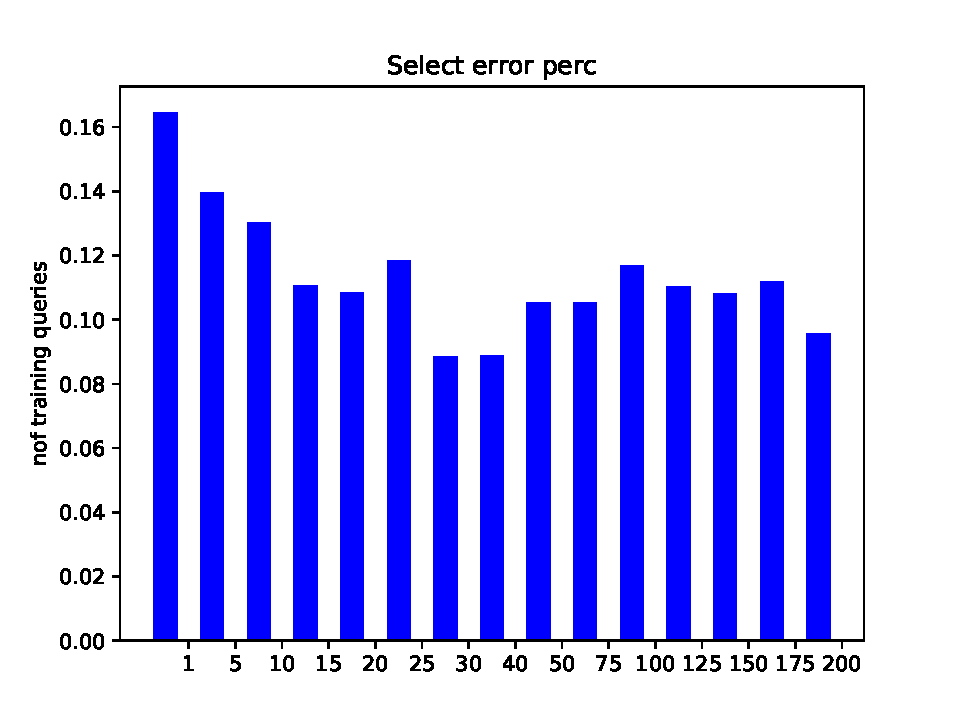
\includegraphics[scale=0.7]{figs/select_error_q6.pdf}
  \caption{Query 6 selection error}
  \label{fig:sel6}
\end{figure}

\end{document}
